\documentclass{article}

\usepackage{epcc}
\usepackage{graphics}
\usepackage{booktabs}
\usepackage{mathrsfs}

\renewcommand{\labelenumii}{\theenumii}
\renewcommand{\theenumii}{\theenumi.\arabic{enumii}.}
% this will make nested numbering all arabic numbers

% This example file shows how a report can be laid out using Latex. It
% does not use any special local features so should be portable to other
% places.
% 
% When producing draft copies of a thesis you may want to print only
% selected pages of the thesis. To do this use the command
% 
% dvips -f -p 4 -n 3 myfile.dvi | lpr
% 
% where -p 4 means start printing at page 4 (ie the page that will be
% numbered 4, not necessarily the 4th page) and -n 3 means print 3 pages.
% This example will print pages 4, 5 and 6.
% 
% If you want to print the report and also save paper you can print more
% than one page on each sheet of paper. Use the command
% 
% dvips -f myfile.dvi | psnup -2 | lpr
% 
% to print 2 pages per sheet. psnup can take values 2, 4, 8, or 9.
%
% To produce a PDF version you can create a PostScript copy first
%
% dvips -f myfile.dvi > myfile.pdf
%
% and then convert it
%
% distill myfile.ps
%
% or you can go straight to PDF
%
% pdflatex myfile
%
% Note that pdflatex expects all included figures to be in PDF too. See
% the includegraphics command below.


% This document contains many cross-references and forward references,
% eg in constructing a table of contents, so Latex may need to be run
% twice to get all the references correct. If you need to run Latex twice
% you may get the warning:
% 
% LaTeX Warning: Label(s) may have changed. Rerun to get cross-references right.


\begin{document}

\pagenumbering{roman}

\title{Project Preparation Report\\Bayesian Inference Using Sequential Monte-Carlo Algorithm for Dynamic System Models}
\author{Chaolin Han}
\date{\today}

\makeEPCCtitle

\newpage

\tableofcontents

% \newpage

% \section*{Acknowledgements}

% This template is a slightly modified version of the one developed by
% Prof. Charles Duncan for MSc students in the Dept. of Meteorology. His
% acknowledgement follows:

% {\em This template has been produced with help from many former students who
% have shown different ways of doing things. Please make suggestions for
% further improvements.}

% \section*{Note}

% This template was originally created for a full MSc dissertation.
% Although I have modified the format slightly (eg there are no separate
% chapters), I have not substantially changed the text or the advice
% appearing in the \LaTeX comments (source lines beginning with \%). You
% should therefore be aware that for a shorter report you may
% not need to go into as much detail as indicated here. For example, you
% might not need to include any acknowledgements and any reference list is
% likely to be very short.



\newpage
\pagenumbering{arabic}

\section{Introduction}

This report focuses on the work in the preparation phase of 
MSc High-performance Computing with Data Analysis Dissertation Project. 
The project is built around 
a biological dynamical systems model with parameter estimation and model comparison 
being the
primary tasks. The complex interactions between several cells and molecules
in zebrafish spinal cord regeneration is the modelling target.

Previous dissertation review section gives comments on the content 
and presentation of a dissertation report. The background of this project is 
introduced in detail regarding several aspects of the project with the motivation
and related literature discussed. 
The preliminary work includes background 
research, literature review, tools and techniques research and their results 
are illustrated. The final project 
proposal and workplan breakdown are given with regards to the conclusion from 
background research and discussion with supervisors, together with a 
estimated project timeline. Risk analysis and possible 
outline of dissertation report are also addressed.

The project aims at the parameter estimation and model comparison. As a kind of 
computational Bayesian inference methods, Approximate 
Bayesian computation (ABC) approaches will be used to estimate parameters of mathematical models and
compare our model with alternative ones. A parallel implementation is of our interests 
and performance data and inference outputs from ABC will be analysed then to evaluate the result.


\section{Previous Dissertation Review}

The reviewed previous dissertation is {\em Modelling Room Acoustics with a 
GPU} by Jacob Josiah Webber, finished in August 2017.
\subsection*{Summary}

Finite-difference time-domain (FDTD) techniques are introduced to numerically solve an acoustics model. The sound will be affected by the room it is in. The solution of wave equations of the sound can be computationally approximated using FDTD. It is a traditional simulation job for GPU. To improve the performance, the author proposed a ‘bounding box’ method, whose accompanied data structure significantly reduced memory usage and resultant simulation computation time is saved.

\subsection*{Does the dissertation adequately explain the context in which the problem is set?}

The motivation is addressed in Chapter 1 (Introductions) and the first part of Chapter 2. It briefly introduced together with its performance concerns. More details could be added to describe the meaning of this modelling mission and performance optimisation mission with relevant application or implementation examples given to clarify it.

The background and literature review is represented adequately in details. Section 2.1 derived formulas about acoustics wave, applied finite-difference on them and obtained an iterative propagation computation equation (Equation 2.15) which is the operation o the numerical modelling. Related boundary conditions and stencilling operations are also properly described. Later sections (2.3 and 2.4) addressed the GPU-based parallelisation and FDTD performance issues in the acoustics modelling context.

The background and literature review section is well structured and addressed and explains the problem background in a way that readers without much-related background knowledge (e.g. acoustics, GPU structures) could understand it.

\subsection*{Has the student adequately explained the scope of the problem, the approach that they would take, how success would be measured and reflected on the outcomes?}

The aim of the project is to propose a new method and improve the modelling performance. To address the benefits of the proposed method, the author gave both theoretical  (section 3.3)and experimental (section 5.2) analysis to prove its effectiveness. The software development process (section 4.2) and theoretical derivation and implementation of the ‘bounding box’ method (2.4.1 and 3.2) are reasonable and adequate.

The reproducibility is achieved by giving the specific hardware platforms (NVIDIA K20 GPU server) and its environment (Appendix B), as well as source code and building instructions. As the author addressed in section 5.3, the replication of the program should output a consistent timing results to ones in Table 5.1 and 5.2.

In regard of the limitations, as stated in the conclusion section, ‘particular effort was made to avoid choosing rooms that were overly suited to the new method’; however more test case should be given to make the results more convincing. Another limitation has been stated in the introductory paragraphs of Chapter 4, where experimentation and results analysis are not fully explored due to lack of time.

The overall outcome is satisfying as it matches the theoretical prediction and the improvement is significant compared to previous method, regardless of the above limitations. 

\subsection*{Quality of presentation}
The language is accurate and descriptions of the theories, designs and implementations are clear to follow.

The listed figures are informative. E.g., Figure 2.1 gives clear representation of the stencilling operations, and Figure 3.1 is a suitable example to illustrate the theories.

The dissertation is well structured such that the process of the project and the works in each stage of the project are included. The tables and algorithm blocks are all represented in clear academical forms, so do their placement and alignment. The formulas and equations, algorithm blocks and figures are all consistently numbered and referred properly.

The references are managed in a consistent manner and are correctly referred when needed. The appendices include original unsummarised data, code and GPU device information which provide meaning supplement when readers want to check some details not mentioned in the main body. However some other content should also be presented here, e.g. implementation environment, experiment input (boundary settings) and benchmarking tools/methods.

\section{Background and Literature Review}

Mathematical models are helpful in resolving complex interactions in real-life 
dynamical systems. The project will use a mathematical model to represent 
zebrafish spinal cord regeneration process, then determine its parameter 
estimation and compare it with alternative models.

Zebrafish is one kind of freshwater fish that is widely used in scientific 
research for its regenerative abilities. Zebrafish can regenerate their spinal 
cord after injury. Tsarouchas et al.\cite{ref:Tsarouchas} revealed how the immune system 
responds to 
allow axons of nerve cells growth across the lesion site. The experiments showed 
evidence that several kinds of immune cells and cytokines play determinative 
roles in regulating inflammation and repair. Cytokines are small proteins 
secreted by certain cells to pass signals across cells. The regeneration 
process is controlled by two cytokines, Il-1$\beta$ and Tnf-$\alpha$. Generally, 
Il-1$\beta$ 
inhibits the regeneration while Tnf-$\alpha$ promotes it, both of which are 
dynamically controlled by mainly two kinds of immune cells (i.e. macrophage, 
neutrophil). Based on these experimental results the initial 
hypothesis is proposed that the repair process are dynamically controlled by 
interactions between these cells and cytokines. Figure \ref{fig:1} illustrates the 
basic interactions.


\begin{figure}

\begin{center}
\resizebox{0.60\hsize}{!}{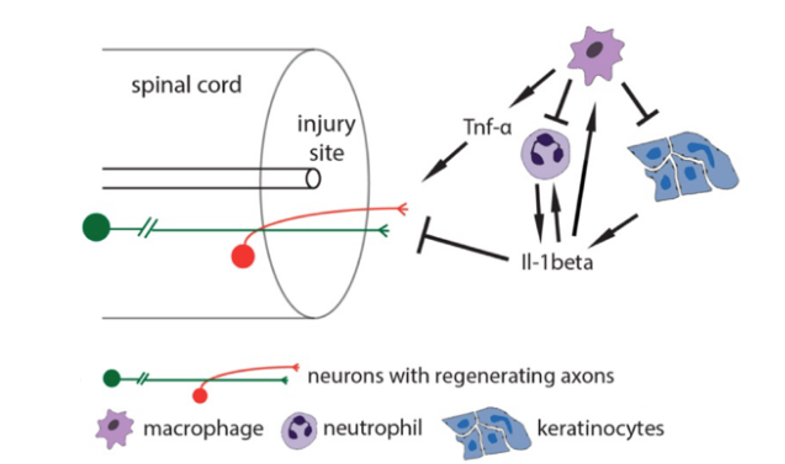
\includegraphics{fig/fig1}}
\end{center}

\caption{Interactions in zebrafish spinal cord regeneration, proposed by Tsarouchas 
et al\cite{ref:Tsarouchas}. Lines ended with an arrow indicate promotion and lines 
ended with a short segment indicate inhibition}
\label{fig:1}

\end{figure}

Mathematical models used to describe complex interactions of dynamical systems 
are usually in the form of differential equations. Analytically solving differential 
equations is not always feasible and the solution can be extremely complicated 
especially for complex systems, so often dynamical system models are solved 
numerically to generate data, which can be compared with real data and determine 
model error. According to our hypothesis an initial ordinary differential equation 
system can be built by describing the dynamics of number or concentration of immune 
cells and cytokines. The initial equations shown in (\ref{eq:1}) are preliminary equations 
that represent the dynamical model, which might be adjusted or calibrated according 
to modelling results and real-world data. 

In (\ref{eq:1}), $N$ and $\Phi$ represent the
number of neutrophil and macrophage respectively, $\alpha$ and $\beta$ denotes the
relative concentration of cytokines Tnf-$\alpha$ and Il-1$\beta$. 
$\lambda$, $\kappa$, $\mu$, $s$, $i$ and $\nu$ with different subscripts are 
all model parameters i.e. coefficient in the interactions.

\begin{equation} \label{eq:1}
\begin{array}{l}
\frac{\mathrm{d} N}{\mathrm{d} t}=\lambda_N+\kappa_{N\beta}\beta-\mu_NN-\nu_{N\Phi}N\Phi\\\\
\frac{\mathrm{d} \Phi}{\mathrm{d} t}=\lambda_\Phi+\kappa_{\Phi\beta}\beta-\mu_\Phi\Phi\\\\
\frac{\mathrm{d} \beta}{\mathrm{d} t}=\frac{s_{\beta N}N}{1+i_{\beta\Phi}\Phi}-\mu_\beta\beta\\\\
\frac{\mathrm{d} \alpha}{\mathrm{d} t}=s_{\alpha\Phi}\Phi-\mu_\alpha\alpha
\end{array}
\end{equation}

A mathematical model will introduce parameters (e.g. $\kappa$, $\mu$ ,etc in (\ref{eq:1})), which are to be determined to 
give a specific model using observed data. A traditional method to find the best desired parameter sets 
is to apply an optimisation-based fitting, where the discrepancy of the model’s 
predictions and experimental data is minimised. Alternatively, by adopting Bayesian 
inference, we can focus on the experimental data and try to infer the parameter sets. 
Many approaches have been proposed and used in the area of systems biology\cite{ref:Stumpf}. Compared 
to optimisation-based fitting methods, Bayesian inference approaches can relieve the 
concerns of over-fitting and local optima. It focuses on posterior distribution which 
represents parameters’ ‘uncertainty’ given the observation data. As Bayes rule 
stated, the posterior distribution $p(\theta|D)$ is proportional to product of likelihood and 
prior
\begin{equation} \label{eq:2}
p(\theta|D)\propto l(\theta|D)p(\theta)
\end{equation}
where $\theta$ denotes parameter vector, $l$ is the likelihood function and $D$ is the observed data.

The prior distribution $p(\theta)$ is given to specify the initial estimates on 
parameters before observing the data; the likelihood is given as conditional 
probability $l(\theta|D)$ which indicates how well the observed data is explained by 
the parameter $\theta$.

% It can be hard to find analytical expression for likelihood, especially in large 
% complex models; instead computational approaches such as Markov Chain Monte Carlo 
% (MCMC)\cite{ref:Gilks} and sequential Monte Carlo (SMC)\cite{ref:Toni} are proposed to 
% solve this problem. 
% These approaches try to approximate the 
% posterior distribution by simulating the data and they are known as approximate Bayesian 
% computation (ABC). S.A. Sisson\cite{ref:Sisson} illustrated that sequential Monte Carlo sampler can 
% be more powerful and efficient than MCMC and traditional ABC rejection methods. 

It can be hard to find an analytical expression for likelihood, especially in large 
complex models. Computational approaches such as Markov Chain Monte Carlo\cite{ref:Gilks} techniques
could be used 
to solve this, where sampling methods are provided to computationally evaluate the likelihood.
Approximate Bayesian computation (ABC) methods are alternative solutions. They are likelihood-free 
methods that simulate data from model and approximate posterior distribution 
instead of evaluating the likelihood. There are several ABC approaches e.g. ABC-rejection, ABC-MCMC
and ABC-SMC (sequential Monte Carlo)\cite{ref:Toni}. S.A. Sisson\cite{ref:Sisson} suggested that sequential Monte Carlo sampler in ABC can 
be more powerful and efficient than ABC-MCMC and traditional ABC rejection methods. 

ABC approaches have been widely used in biology applications due to their 
‘likelihood-free’ feature. In many systems biology models, the likelihood is 
intractable, meaning that it cannot be defined as a function of the 
parameters $\theta$ analytically. Liepe et al.\cite{ref:Liepe} showed a 
successful application of 
ABC-SMC in systems biology 
with a software package ABC-SysBio, where ABC-SMC is used both in parameter estimation and model 
selection.

Parameters of the zebrafish spinal cord regeneration model can be estimated 
using ABC-SMC as it is hard to find exact likelihood here and an efficient 
approximation approaches might help us in exploring the uncertainty in parameter 
sets and comparing our model with alternative ones.

% see the man page for dvips for details of the special command which is
% much more powerful than is shown here. It allows offsets in the
% horizontal and vertical and scaling in x and y.

% choosing suitable values for offset and scale can be a tiring matter
% of trial and error.

% note that labels do not need to include a description of the object
% they are labelling but it can be helpful, eg \label{fig:figurename}.


\section{Preliminary Investigations}

Preliminary works include background material study and tools research, which aims to build a concrete start of the project and explore the uncertainty and suitability of tools.

\subsection{Background Research}

The two key background papers\cite{ref:Tsarouchas,ref:Liepe} were studied firstly. 
Tsarouchas et al.\cite{ref:Tsarouchas} illustrated 
the biology process (zebrafish spinal cord regeneration after injury) that we want to 
model and introduced the dynamic controls within the process in details. As 
shown in the paper the process requires related biology 
background knowledge, especially in immunology, thus related necessary background
materials were studied to form a more comprehensive understanding and could help in 
future analyse of results. The other background paper focuses on the algorithms that 
are expected to be implemented in the project. More materials related to Bayesian 
inference were studied, including tutorials, books and articles. Basic theories of 
Bayesian inference and practical examples were studied with several ABC tutorial examples 
practised to improve understanding. Other background materials include papers on 
ABC-SMC algorithm, including the theory, implementation steps and comparison with 
other ABC algorithms.

The mathematical models were also preliminarily studied, with concerns over model 
building, data processing and solving. Ordinary differential equation computational 
solution and its solver were reviewed in preparation for the future actual 
implementation.

The background research is the most important work in the preparation phase, 
as it converted the first impression and interests of the project into concrete 
knowledge in the biology and statistical inference basis such that the mission, 
risks and challenges of the project could be discussed and analysed; it also 
ensured an easier technically start of the project.

\subsection{Tools Research}
Besides the background research, tools that might be used in the project, mainly 
the packages and libraries, were studied, compared and evaluated.

There are currently varies of tools and softwares that implement ABC-SMC. A desirable tool should take many technical aspects into account, e.g. working environment, mathematical models solvers, parallelisation support and reliability.

ABC-SMC is expected to be applied in Python or R languages, as most of the published packages are implemented on these two languages; further studies may use other languages if a more suitable software package for that is found or we need to build our own code for optimising.

The studied packages are listed in Figure \ref{fig:2}. Their user guidance, 
documentations (if exist) are viewed, from which their features are concluded 
in a note (taskPackages.md under tasks directory in project repository);
their main features are listed below. 

\begin{figure}

	\begin{center}
	\resizebox{1.00\hsize}{!}{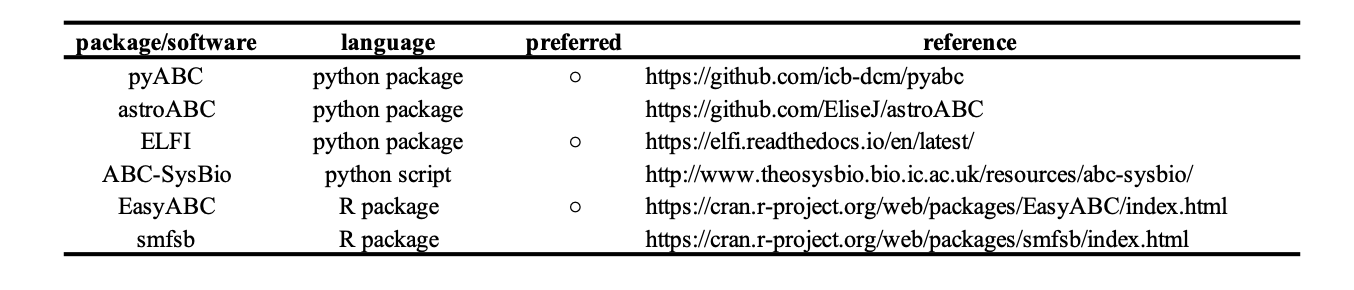
\includegraphics{fig/fig2}}
	\end{center}
	
	\caption{Studied packages}
	\label{fig:2}
	
	\end{figure}


\begin{enumerate}
	\item pyABC
	\begin{itemize}
		\item It has built-in support for multiple types of parallelisation, e.g., 
		multicore processing and distributed cluster

		\item Stored runs can be resumed
		
		\item Several built-in visualisation for the results are provided
	\end{itemize}

	\item astroABC
	\begin{itemize}
		\item It supports parallel sampling using MPI or multiprocessing
		
		\item Every run of the sampling can be paused and resumed later
	\end{itemize}

	\item ELFI
	\begin{itemize}
		\item It allows user to connect to \texttt{ipyparallel} for more parallelisation options
		
		\item It uses directed acyclic graph as input model; a conversion is needed before implementation
	\end{itemize}

	\item ABC-SysBio
	\begin{itemize}
		\item It has experimental CUDA accelerated parallelisation support
		\item It is specially designed for systems biology applications
		
	\end{itemize}

	\item EasyABC
	\begin{itemize}
		\item It supports multicore parallelisation
		
		\item Several different sequential algorithms are offered
	\end{itemize}

	\item smfsb
	\begin{itemize}
		\item It provides simple and basic output of parameter estimations
	\end{itemize}

\end{enumerate}


Some examples given in their documentations have been practised to explore the details and features of ABC-SMC algorithm in these packages and determine which of them meet our requirements. The three preferred packages are pyABC, EasyABC and ELFI. All of them are well documented and support different kinds of parallelisation; other features include support for built-in visualisation, pause-and-restart and easy to use. The choice is limited in the preliminary practise and may be changed accordingly in the future practical implementation as more packages will be studied.

Tools research provides grounded comprehension and conclusion on packages 
choosing in this project and finds the initial tools to start with. More 
tools will be studied and possibly used in the future.

\section{Final Proposal}

The project research consists of six parts. The first two parts are preparation work that would result in a mathematical model to implement our algorithms. Part 3, 4 and 5 are the practical session including several experiments and implementations to explore and analyse the model. The last part is to organise the works into report and dissertation.

\subsection{Background Research and Project Preparation}

This part focus on the preparation of the project, including background reading, tools research and regular discussion with supervisors. It will build a concrete ground to start the later tasks. Most of the work have already been done.

\subsection{Dynamical System Modelling}

Non-linear differential equations will be adapted to represent the dynamic system of zebrafish spinal cord regeneration process. Under the hypothesis1, there are complex interactions between two types of cytokines and three types of cells at the wounded site and the expected mathematical model representing by ODE systems will be built to describe these interactions.

\subsection{Parameter Estimating}

The parameters in the ODE system will be estimated using experimental data1. ABC-SMC will be applied to approximate the posterior distribution of parameters and produce reliable parameter estimates of the model. A distance function will be built to measure the discrepancy between the model and simulated data before applying the algorithm, together with coping with missing data in certain time points.

As the SMC sampling process is computation-intensive and thus time-consuming, a parallel sampling technique will be of our interest. 

\subsection{Results Interpretation and Analysing}

This part focuses on the evaluation of the parameterised model and analysis of the SMC results. Inference results will be tested using synthetic data and used to evaluate how well the model fits the data and how much confidence we have on the parameter estimates.

\subsection{Model Comparison}

ABC-SMC can also be implemented to compare our model with alternative ones. Similar procedures will be applied to model candidates and result in an approximation of each model’s marginal distribution, which could be the main criteria for our model selection.

\subsection{Performance Analysis}

The performance data of the sampling process will be analysed to reveal performance of the parallelisation implementation, including parallel speedup and efficiency. Trade-offs between cost, runtime and energy will also be discussed.

\subsection{Dissertation and Report Writing}

A project study report and final dissertation will be written to address all works and results in the project research process.

\subsection{Estimated Computational Resources Usage}

The computational resources usage estimation is a provisional rough estimation, 
which can be changed as the implementation and performance test proceeds.

\textbf{Cirrus}

Most of the computational work in this project is expected to be deployed on Cirrus.
\begin{itemize}
	\item CPU hrs needed (standard compute nodes): 7200 CPUh (2 hrs per run $\times$ 
	36 cores$\times$ 100 runs)
	\item Disk storage needed: 10 GB, including data and softwares
	\item Access to GPU compute nodes is also needed for possible parallelisation using CUDA
\end{itemize}

\section{Workplan}

Each part of the project research is planned as followed. The first stage is to prepare for the project in Semester 2 and possibly in the Easter holidays; the second stage will start at 18 May when the last examination ends.

\begin{enumerate}
	\item Background Research and Project Preparation, Dynamical System Modelling
	
	$\bullet$ Start time: 21/01/2020
	
	$\bullet$ Duration: 8 weeks
	
	$\bullet$ The later Easter holidays could be used to do more research

	\item Parameterising
	
	$\bullet$ Start time: 18/05/2020
	
	$\bullet$ Estimated duration: 7 weeks

	\item Results Interpretation and Analysing
	
	$\bullet$ Start date: 22/06/2020
	
	$\bullet$ Estimated duration: 5 weeks

	\item Model comparison
	
	$\bullet$ Start date: 15/06/2020
	
	$\bullet$ Estimated duration: 5 weeks

	\item Performance Analysis 
	
	$\bullet$ Start date: 13/07/2020
	
	$\bullet$ Estimated duration: 2 weeks

	\item Dissertation and report writing
	
	$\bullet$ Start date: 20/07/2020
	
	$\bullet$ Estimated duration: 5 weeks

\end{enumerate}

The Gantt chart is shown in Figure \ref{fig:3}. The two stages are separately listed.

\begin{figure}

	\begin{center}
	\resizebox{0.80\hsize}{!}{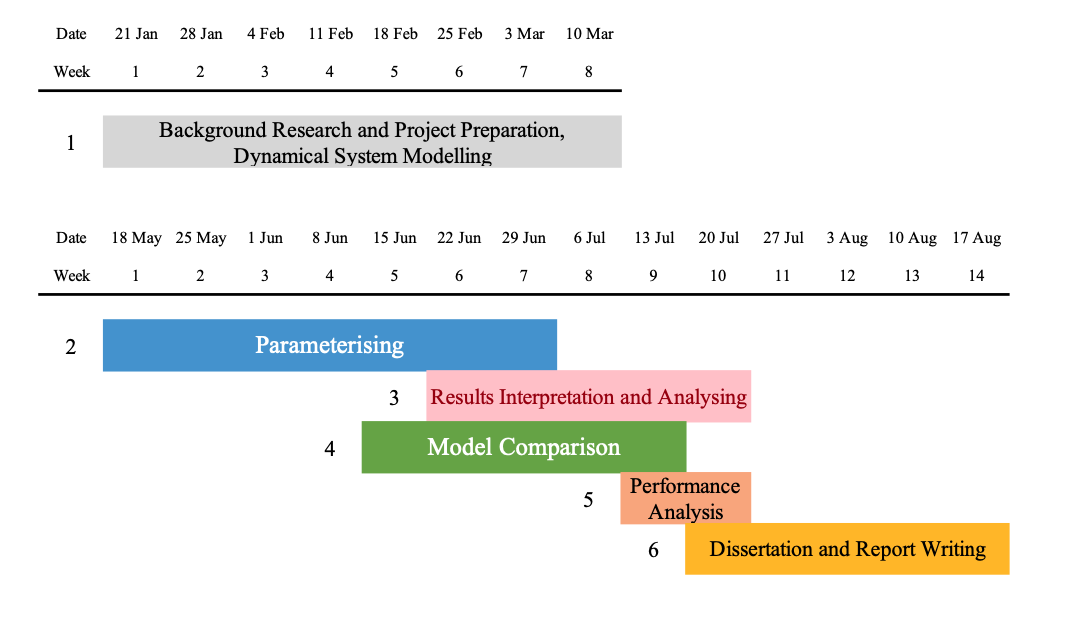
\includegraphics{fig/fig3}}
	\end{center}
	
	\caption{Workplan Gantt chart}
	\label{fig:3}
	
	\end{figure}


\section{Risk Analysis}

Possible risks and challenges are addressed in this section. These risks are concluded from the preliminary researches. Though we tried to predict and evaluate all risks in the project, new risks may appear as the project proceeds.

\subsection{Technical Problems}

\textbf{Tools/software problems} 

\begin{itemize}
	\item There could be unforeseen bugs in the code of the tools or software that are used in the project; softwares may crash, leading to possible data damaging. It is usually unpreventable. 

	Probability: moderate
	
	Mitigation: in this case, we may need to find and fix the bug, switch tool/softwares and/or make a data protection plan to reduce the impact.
	
	\item There could be problems in the implementation environment where the compatibility is our main concern. The implementation may require certain environment conditions (e.g. operating system, compiler version, dependencies, etc) to be performed, or they could be incompatible with the hardware (e.g. CUDA acceleration and multithreading). 
	
	Probability: high
	
	Mitigation: we have studied a variety of packages (section 4.2) to ensure that we have alternatives when it is necessary to switch tools, and will take more tools into the backup plan. Another solution is to change or built the required environment if applicable, i.e. switching OS, compile environment or hardware platform.

	\item The worst case could be that we may need to write our code to implement the ABC-SMC algorithm and complete the rest study, which would heavily increase the workload.
	
	Probability: low
	
	Mitigation: The workplan should be adjusted once it happens to ensure more time devoted to algorithm code and debug process. The rest work may be simplified.

\end{itemize}

\textbf{Hardware problems} 

\begin{itemize}
	\item Hardware failures and hardware unavailability could intrude considerable impact on the project process. Hardware failure may cause data damaging; hardware unavailability may break the estimated workplan.
	
	Probability: low
	
	Mitigation: a regular data backup should be planned where experiments records, results and configurations should be well protected. In this case to proceed the project we may need to seek for hardware alternatives.
\end{itemize}

\subsection{Parallelisation Concerns}

\begin{itemize}
	\item The project seeks to implement a parallel sampling. The first risk could be that different tools use different parallel techniques targeting different hardwares, where the parallel performance comparison across hardware is a problem.
	
	Probability: high
	
	Mitigation: more study on the cross-platform benchmark should be conducted to give a reasonable comparison of performance.

	\item Another risk can be the tricky parallel implementations, as there are different parallel systems with different configuration; it may cost time to find which kinds of implementation would work before we proceed to parallel performance analyse.
	
	Probability: moderate
	
	Mitigation: more investigation of the parallel implementations should be performed, which can reduce the effort in finding working schemes along with investigations in section 4.2.

	\item The execution time of parameterising using ABC-SMC is mainly determined by problem size and sampling parameters (number of generations, tolerance sequence and population size); it may cost time to obtain a reasonable parameter input that avoids long execution time and in the meantime give precise results. Another trade-off we may face could be the common scalability trade-offs where a suitable scale-up is to be discussed.
	
	Probability: high
	
	Mitigation: It is usually unavoidable. To minimise the cost and effort a plan on the implementation experiment should be made and discussed where only necessary experiment should be conducted and redundant parameter space enumeration should be avoided. 
\end{itemize}

\subsection{Modelling}

\begin{itemize}
	\item The main risk in the modelling process is model misspecification. 
	
	Probability: moderate
	
	Mitigation: we may need to calibrate our model or adopt another model. These changes could consequently affect all later works in parameterising and analysis and the workplace should be adjusted accordingly.
	
	\item There is also risks in experiment data processing: variables are measured in different time steps and data on gene expression uses different scales from the differential equations. These problems will introduce some difficulties in the model fitting.
	
	Probability: high
	
	Mitigation: the processing methods should be studied and backup plan should be made to enable a successful fitting.
\end{itemize}

\subsection{Other Risks}

As far as this project concerns, certain cases of force majeure could affect the project progress which are low in probability. It should be noted that the current Coronavirus epidemic could affect some part of the project process, e.g. supervision meetings and access to certain physical resources.

The project may face failure, e.g. undesirables results, critical technical problems and running out of time. These failures should be noticed as early as possible through the risk analysis and management throughout the project time and be avoided as much as we can.

\section{Outline of the Dissertation Report}

A possible outline of the Dissertation Report is structured as below.

\begin{enumerate}
	\item Introduction
	\item Background and Literature Review
	\begin{enumerate}
		\item Zebrafish spinal cord regeneration
		\item Mathematical modelling
		\item Bayesian Inference
	\end{enumerate}
	\item Modelling
	\item Design and Implementation
	\begin{enumerate}
		\item Parameter estimation
		\item Model comparison
		\item High-performance implementations
	\end{enumerate}
	\item Results and Analysing
	\begin{enumerate}
		\item ABC-SMC results
		\item Performance analysis
		\item Discussions
	\end{enumerate}
	\item Future Works
	\item Conclusions
\end{enumerate}

\pagebreak
\begin{thebibliography}{100}

\bibitem{ref:Tsarouchas} Tsarouchas, T.M., Wehner, D., Cavone, L., Munir, T., Keatinge, M., Lambertus, M., Underhill, A., Barrett, T., Kassapis, E., Ogryzko, N. and Feng, Y., 
2018. Dynamic control of proinflammatory cytokines Il-1$\beta$ and Tnf-$\alpha$ by macrophages in zebrafish spinal cord regeneration. Nature communications, 9(1), pp.1-17.

\bibitem{ref:Stumpf}Stumpf, M., Balding, D.J. and Girolami, M., 
2011. Handbook of statistical systems biology. John Wiley \& Sons.

\bibitem{ref:Gilks}Gilks, W.R., Richardson, S. and Spiegelhalter, D., 
1995. Markov chain Monte Carlo in practice. Chapman and Hall/CRC.

\bibitem{ref:Toni}Toni, T., Welch, D., Strelkowa, N., Ipsen, A. and Stumpf, M.P., 
2009. Approximate Bayesian computation scheme for parameter inference and model selection in dynamical systems. Journal of the Royal Society Interface, 6(31), pp.187-202.

\bibitem{ref:Sisson}Sisson, S.A., Fan, Y. and Tanaka, M.M., 
2007. Sequential monte carlo without likelihoods. Proceedings of the National Academy of Sciences, 104(6), pp.1760-1765.

\bibitem{ref:Liepe}Liepe, J., Kirk, P., Filippi, S., Toni, T., Barnes, C.P. and Stumpf, M.P., 
2014. A framework for parameter estimation and model selection from experimental data in systems biology using approximate Bayesian computation. Nature protocols, 9(2), p.439.


\end{thebibliography}


\end{document}

